\documentclass{beamer}


\usepackage[utf8]{inputenc}
\usepackage{amsmath}
\usepackage{amsfonts}
\usepackage{amssymb}
\usepackage{graphicx}
\usepackage{ragged2e}  % `\justifying` text
\usepackage{booktabs}  % Tables
\usepackage{tabularx}
\usepackage{tikz}      % Diagrams
\usetikzlibrary{calc, shapes, backgrounds}
\usepackage{amsmath}
\usepackage{amssymb}
\usepackage{dsfont}
\usepackage{url}       % `\url
\usepackage{listings}  % Code listings
\usepackage[T1]{fontenc}


\usepackage{theme/beamerthemehbrs}

\author[]{Abhishek Padalkar}

\title{Dynamic Motion Primitives}
\subtitle{Research and Development Project}
\institute[HBRS]{Hochschule Bonn-Rhein-Sieg}
\date{\today}
\subject{Test beamer}

% \thirdpartylogo{path/to/your/image}


\begin{document}
	{
	\begin{frame}
	\titlepage
	\end{frame}
	}
	
	\begin{frame}{Motivation}
		\begin{itemize}
			\item Humans \textbf{learn} variety of motions and use them in similar situations. 
			\item Human motions consist of motion primitives. 
			\item Concept of motion primitives can be adopted for robots. 
			\item Learned motion primitives can be combined to do complex task. 
			\item Several approaches are available for learning motion primitives.
		\end{itemize}
	\end{frame}
	
	
	\begin{frame}{Advantages of DMP}
		\begin{itemize}
			\item It is a model free learning approach.
			\item Any arbitrary trajectory can be learned in end-effector space as well as in joint space.
			\item Here learning is linear regression, so it does not need large dataset.
			One trajectory is sufficient ideally.
			\item Trajectories can be scaled in space as well as in time.
			\item Trajectory evolves as robot actually moves along the trajectory. Hence on-line modifications in the trajectory are possible.

		\end{itemize}
	\end{frame}

	\begin{frame}{Formulation of DMP}
		\begin{equation}\label{DMP_1}
		\tau\dot{z} = \alpha_{z}(\beta_{z}(g - y) - z) + f(x)
		\end{equation}
		\begin{equation}\label{DMP_2}
		\tau \dot{y} = z
		\end{equation}
		\begin{equation}\label{forcing_term}
		f(x) = \frac{\sum_{i=1}^{N}\psi_{i}(x)w_{i}}{\sum_{i=1}^{N}\psi_{i}(x)}x(g - y_{0})
		\end{equation}
		where,
		\begin{equation}\label{psi}
		\psi_{i} = \exp(-{\frac{1}{2\sigma_{i}^{2}}(x - c_{i})^{2}})
		\end{equation}
		and,
		\begin{equation}\label{canonical}
		\tau \dot{x} = -\alpha_{x}x
		\end{equation}
		
		[$y, \dot{y}, \ddot{y}$] = kinematic state  \\
		$g$ = goal value \\
		$y_{0}$ = initial value
	\end{frame}
	
	
	\begin{frame}
		\begin{itemize}
			\item Second order differential equation representing \textbf{damped mass spring system.} 
			\item Non-linear term \textit{f(x)} modifies the acceleration and hence characterizes the motion. 
			\item Phase variable \textbf{x} ensures the synchronization between multiple degrees of freedom.  
		\end{itemize}
	\end{frame}

	\begin{frame}{Working of DMP}
		\centering
		\textbf{2D DMP system with no forcing term}
		
		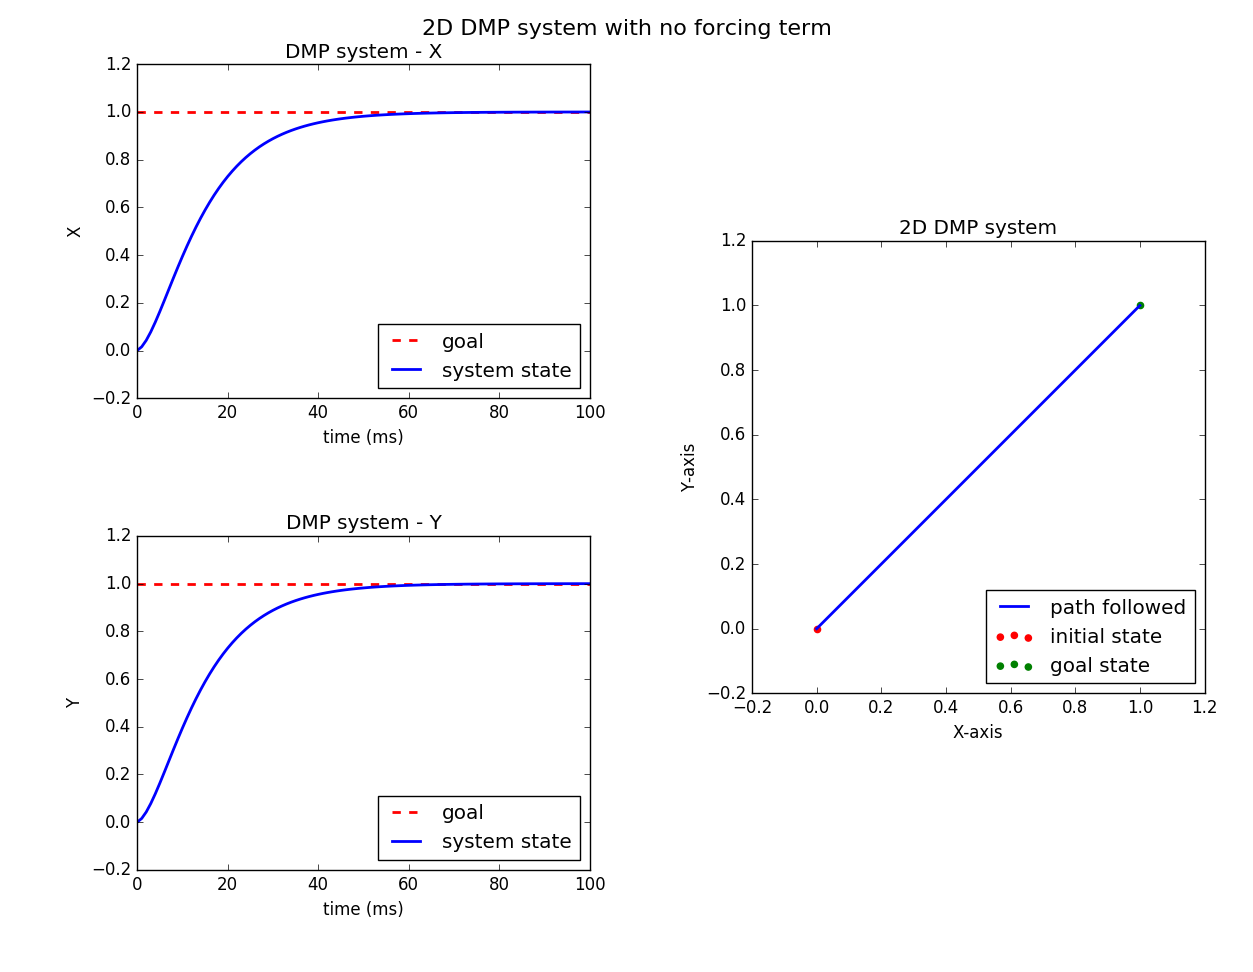
\includegraphics[scale=0.3]{images/dmp_no_f}
	\end{frame}
	
	\begin{frame}
		\centering
		\textbf{2D DMP system with forcing term}

		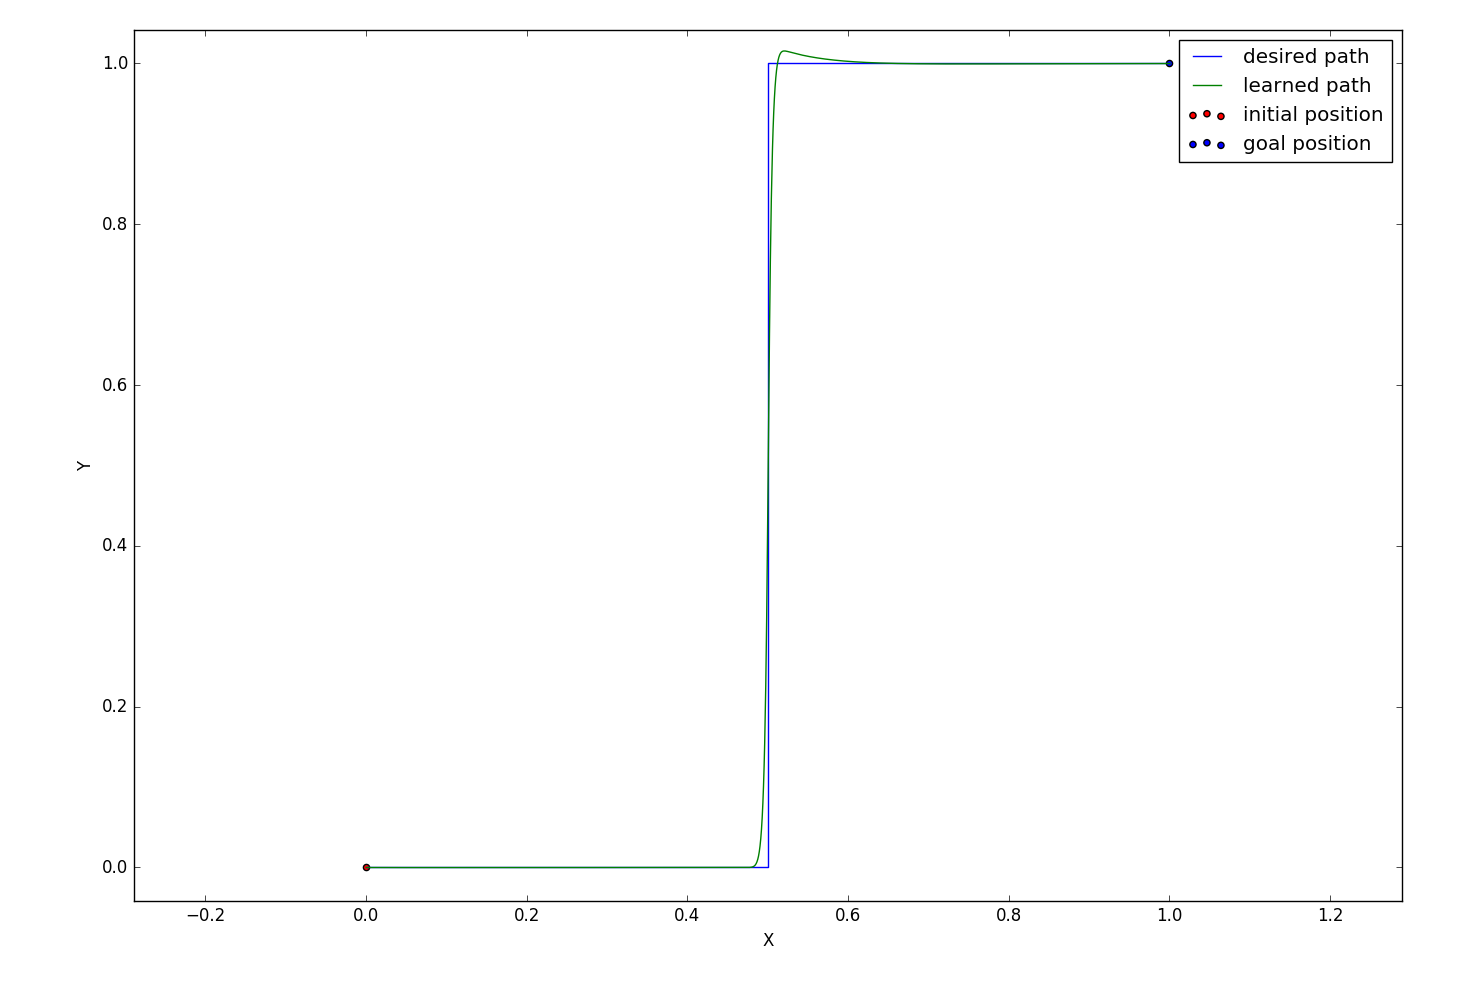
\includegraphics[width=\textwidth]{images/step_f}
	\end{frame}
	
	\begin{frame}
		\textbf{Forcing functions}
		\begin{figure}
			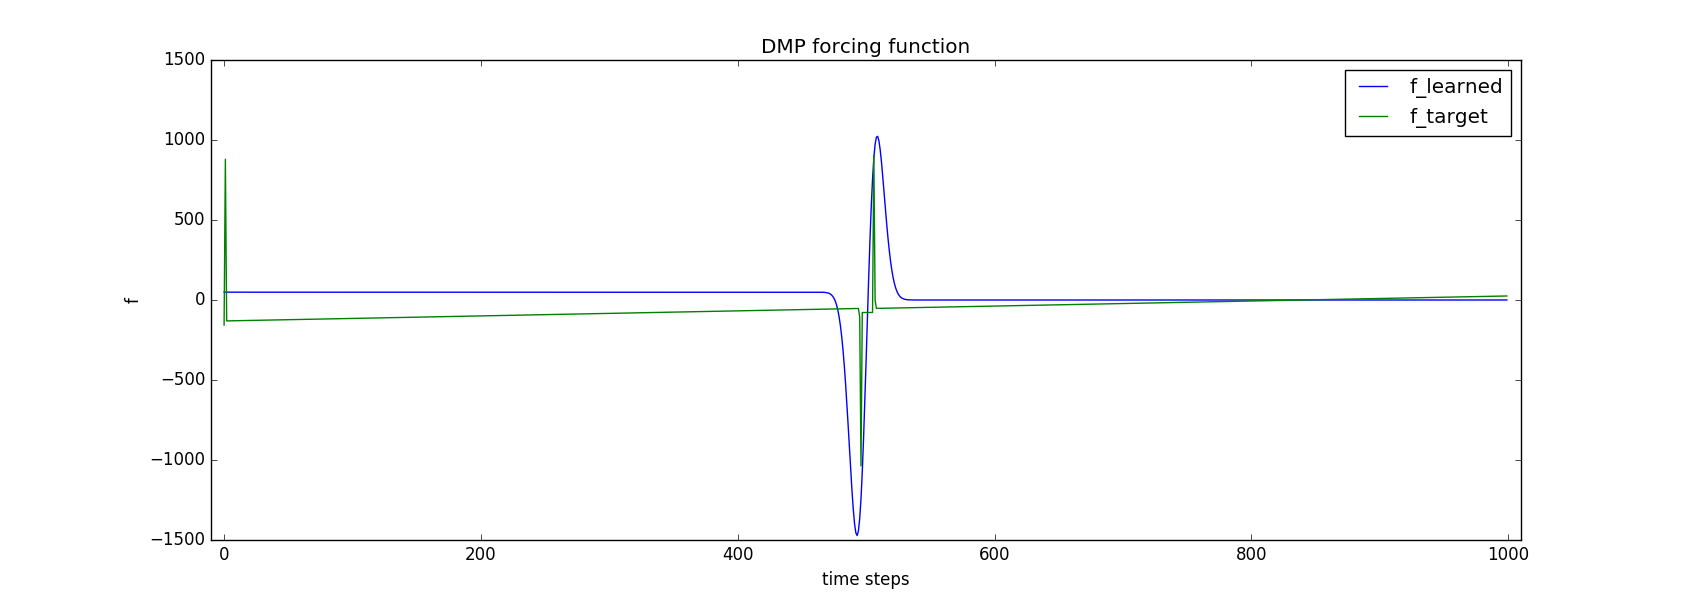
\includegraphics[scale=0.23]{images/f_x}
			\caption{Forcing term - X}
		\end{figure}

		\begin{figure}
			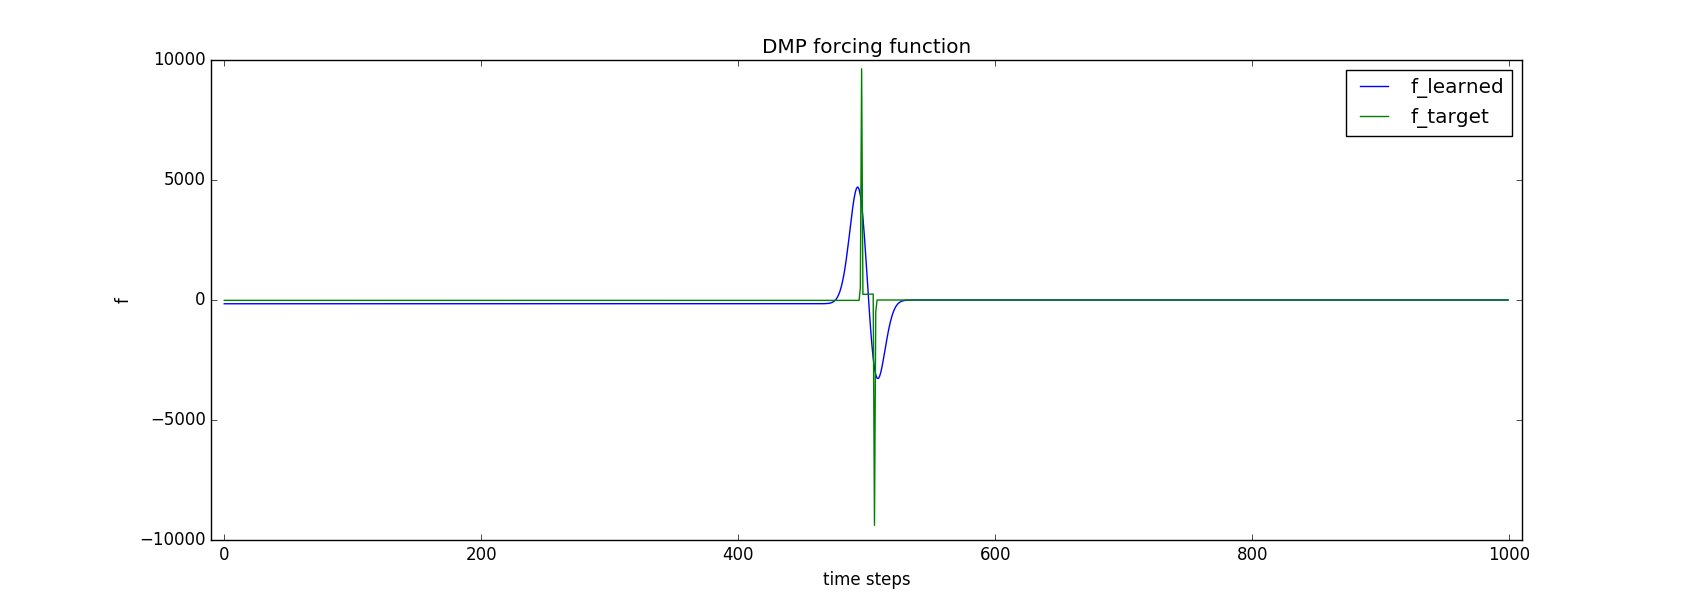
\includegraphics[scale=0.23]{images/f_y}
			\caption{Forcing term - Y}
		\end{figure}
	\end{frame}
	
	\begin{frame}{Analysis of the effects of the parameters used in DMP}
		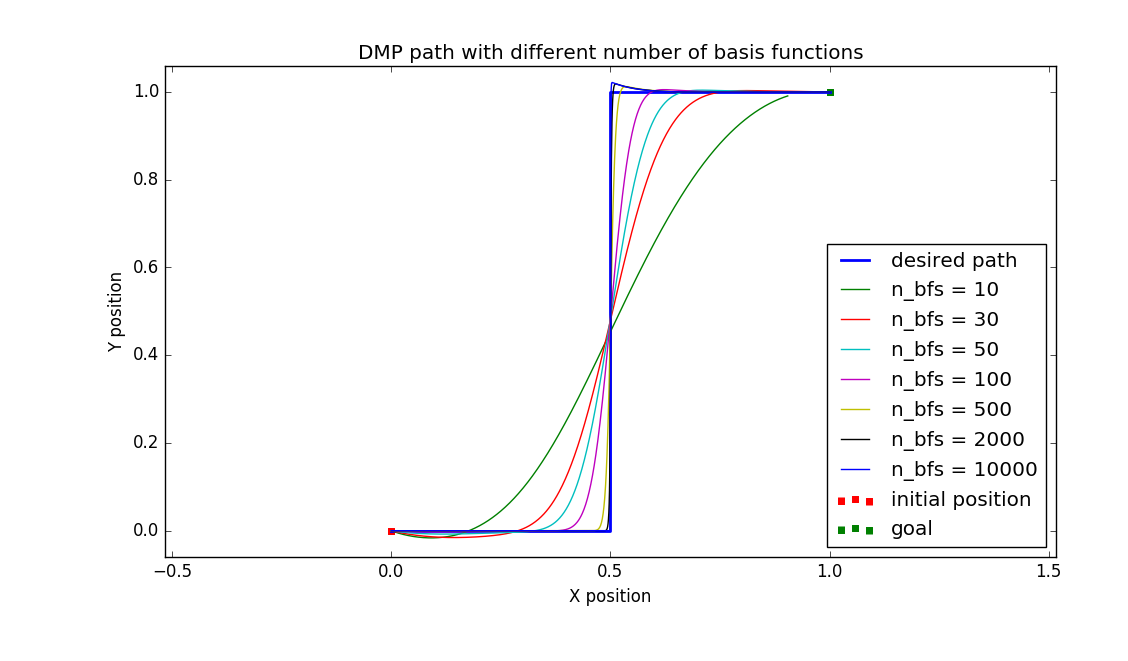
\includegraphics[width=\textwidth]{images/n_bfs_}
	\end{frame}
	
	\begin{frame}
		
		\begin{center}
			\begin{table}[H]
				\begin{tabular}{| c | c | c | c | c | c | c | c |}	
					\hline
					n\_bfs & 10 & 30 & 50 & 100 & 500 & 2000 & 10000\\       
					\hline
					Error & 0.093 & 0.038 & 0.021 & 0.009 & 0.002 & 0.001 & 0.001\\
					\hline
				\end{tabular}
				\caption{Error in mimicking the trajectory}
			\end{table}\label{_n_bfs_e}
		\end{center}
	\end{frame}
	
	\begin{frame}
		\centering
		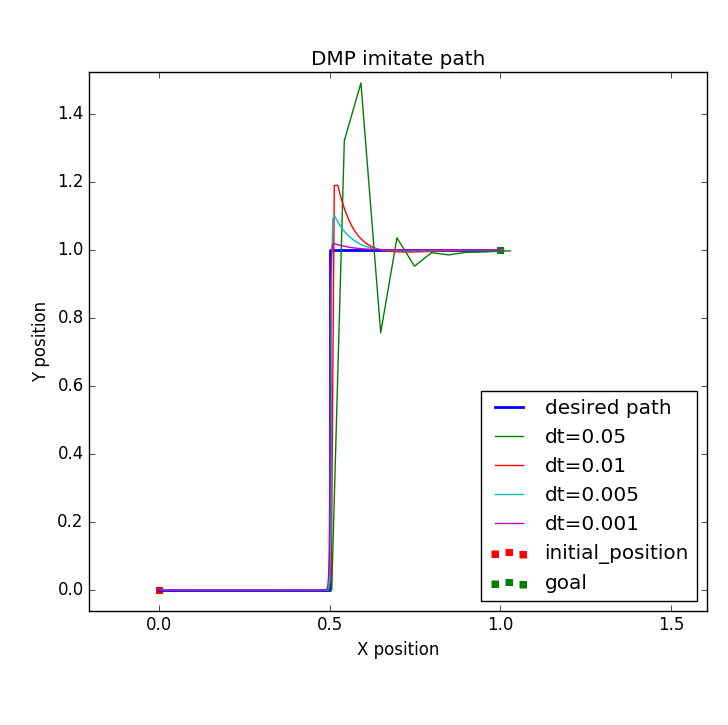
\includegraphics[scale=0.45]{images/dt_}
	\end{frame}
	
	\begin{frame}
		\begin{center}
			\begin{table}[H]
				\centering
				\begin{tabular}{| c | c | c | c | c | c | c | c |}	
					\hline
					Time step size & 0.05 & 0.01 & 0.005 & 0.001 \\       
					\hline
					Error & 0.062 & 0.017 & 0.011 & 0.007 \\
					\hline
				\end{tabular}
				\caption{Error in mimicking the trajectory}
			\end{table}\label{_dt_e}
		\end{center}
	\end{frame}
	
	
	\begin{frame}
		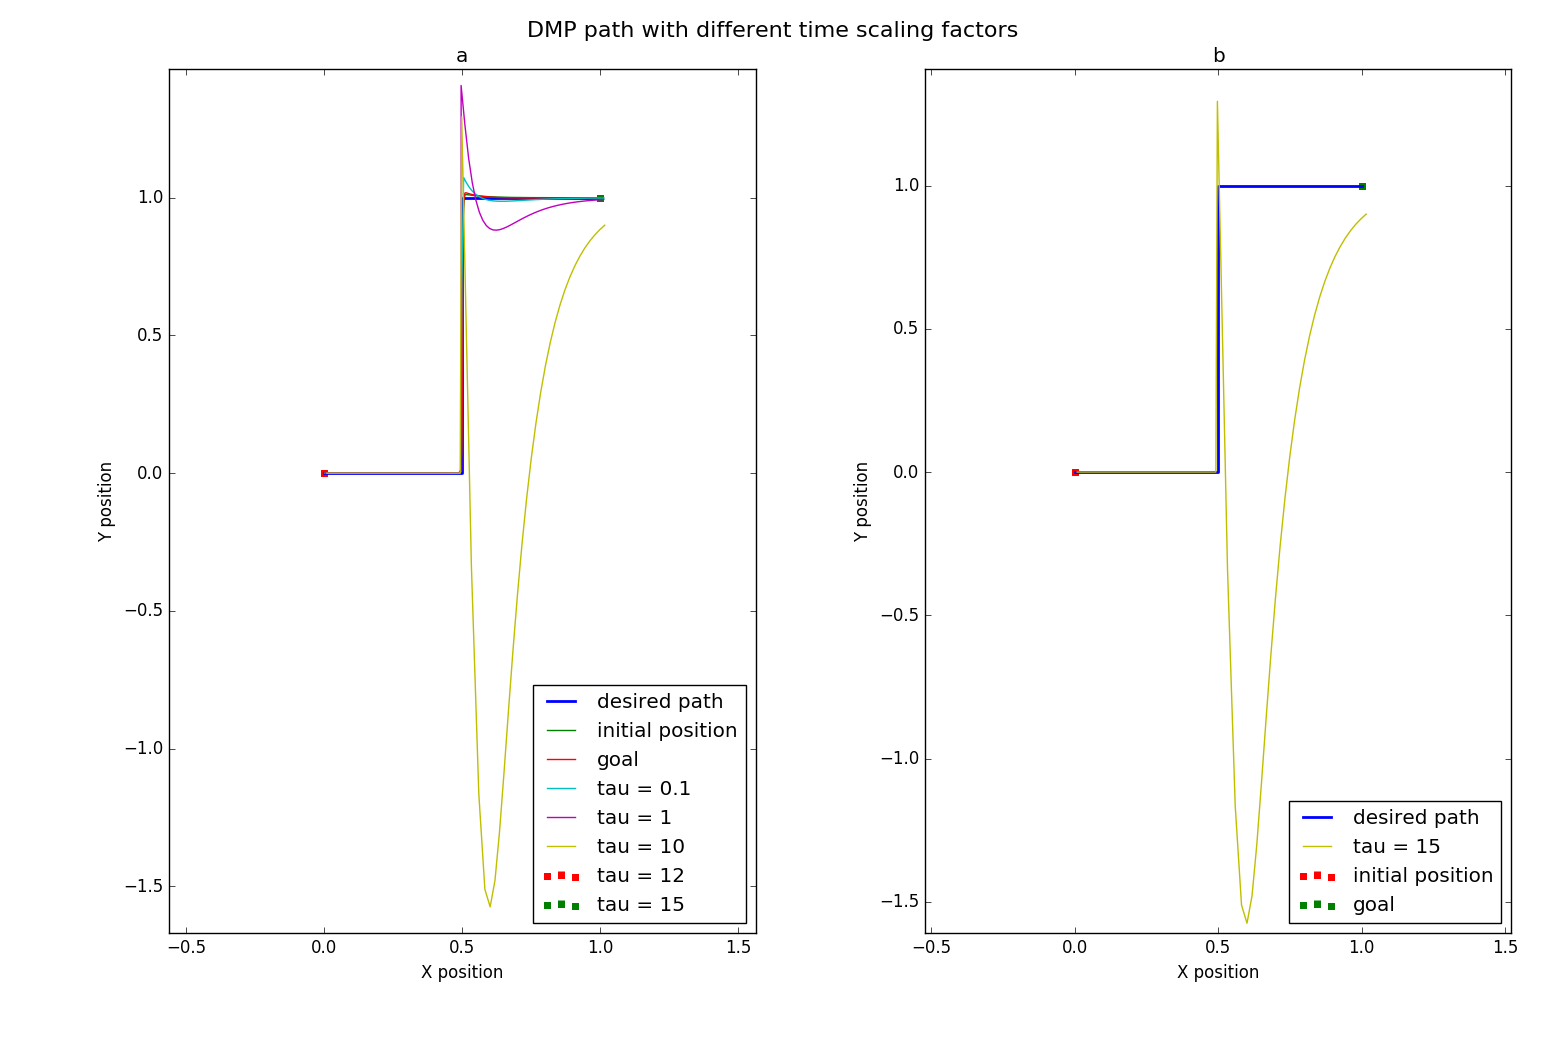
\includegraphics[width=\textwidth]{images/tau_}
	\end{frame}
	
	\begin{frame}
		\begin{center}
			\begin{table}[H]
				\centering
				\begin{tabular}{| c | c | c | c | c | c | c | c |}	
					\hline
					Time scaling factor ($tau$) & 0.1 & 1 & 10 & 12 & 15 \\       
					\hline
					Error & 0.007 & 0.007 & 0.010 & 0.036 & 0.292   \\
					\hline
				\end{tabular}
				\caption{Error in mimicking the trajectory}
			\end{table}\label{_tau_e}
		\end{center}
	\end{frame}
	
	\begin{frame}{Inverse Kinematic Solver}
		\begin{itemize}
			\item Motion is learned in task space. 
			\item Need of inverse kinematic solver to convert Cartesian velocities to joint velocities. 
			\item Limitations of manipulators because of having 5 degrees of freedom.
			\item Weighted Damped Least Square method for calculating joint velocities.
		\end{itemize}	
	\end{frame}
	
	\begin{frame}{Whole Body Motion Control}
		\begin{equation}
		m_{cap} = \frac{(\sigma_{min} - \sigma_{l})}{(\sigma_{h} - \sigma_{l})}
		\end{equation}

		\begin{equation}
		b_{cap} = \frac{(d - d_{l})}{(d_{h} - d_{l})}
		\end{equation}
		
		\begin{equation}
		v_{ee} = m_{cap}.v
		\end{equation} 
		
		\begin{equation}
		v_{b} = (1 - m_{cap}).v
		\end{equation} 

	\end{frame}
	
	\begin{frame}{Experiments}
		\begin{itemize}
			\item 
		\end{itemize}
	\end{frame}
	
	\begin{frame}{Results}
	
	\end{frame}
	
	\begin{frame}{Conclusion}
	\begin{itemize}
		\item learning from demonstration architecture was developed for robot programming.

		\item We provide an intuitive explanation of the working of the dynamic motion primitives. By observing limitations on the motion of the KUKA YouBot manipulator, we developed the concept of using motion policy encoded in DMP for performing whole body motion control. Developed whole body motion control architecture significantly increased the manipulation capabilities of the mobile manipulators KUKA YouBot and Toyota HSR. Whole body motion control has already been integrated into software stack used on Toyota HSR, where it replaces the MoveIt! framework for motion planning. With all these experiments, we gathered enough insights of the working of DMPs for building a library of DMP and use it for performing robotic tasks in RoboCup@Home scenario.
	  	\end{itemize}
	\end{frame}

\end{document}
